Here we provide some further tips.

\mypar{Further general guidelines}

\begin{itemize}
\item For short papers, to save space, I use paragraph titles instead of
subsections, as shown in the introduction.

\item It is generally a good idea to break sections into such smaller
units for readability and since it helps you to (visually) structure the story.

\item The above section titles should be adapted to more precisely
reflect what you do.

\item Each section should be started with a very
short summary of what the reader can expect in this section. Nothing
more awkward as when the story starts and one does not know what the
direction is or the goal.

\item Make sure you define every acronym you use, no matter how
convinced you are the reader knows it.

\item Always spell-check before you submit (to me in this case).

\item Be picky. When writing a paper you should always strive for very
high quality. Many people may read it and the quality makes a big difference.
In this class, the quality is part of the grade.

\item Books helping you to write better: \cite{Higham:98} and \cite{Strunk:00}.

\item Conversion to pdf (latex users only): 

dvips -o conference.ps -t letter -Ppdf -G0 conference.dvi

and then

ps2pdf conference.ps
\end{itemize}

\mypar{Graphics} For plots that are not images {\em never} generate (even as intermediate step)
jpeg, gif, bmp, tif. Use eps, which means encapsulate postscript, os pdf. This way it is
scalable since it is a vector graphic description of your graph. E.g.,
from Matlab, you can export to eps or pdf.

Here is an example of how to get a plot into latex
(Fig.~\ref{fftperf}). Note that the text should not be any smaller than shown.

%\begin{figure}\centering
%  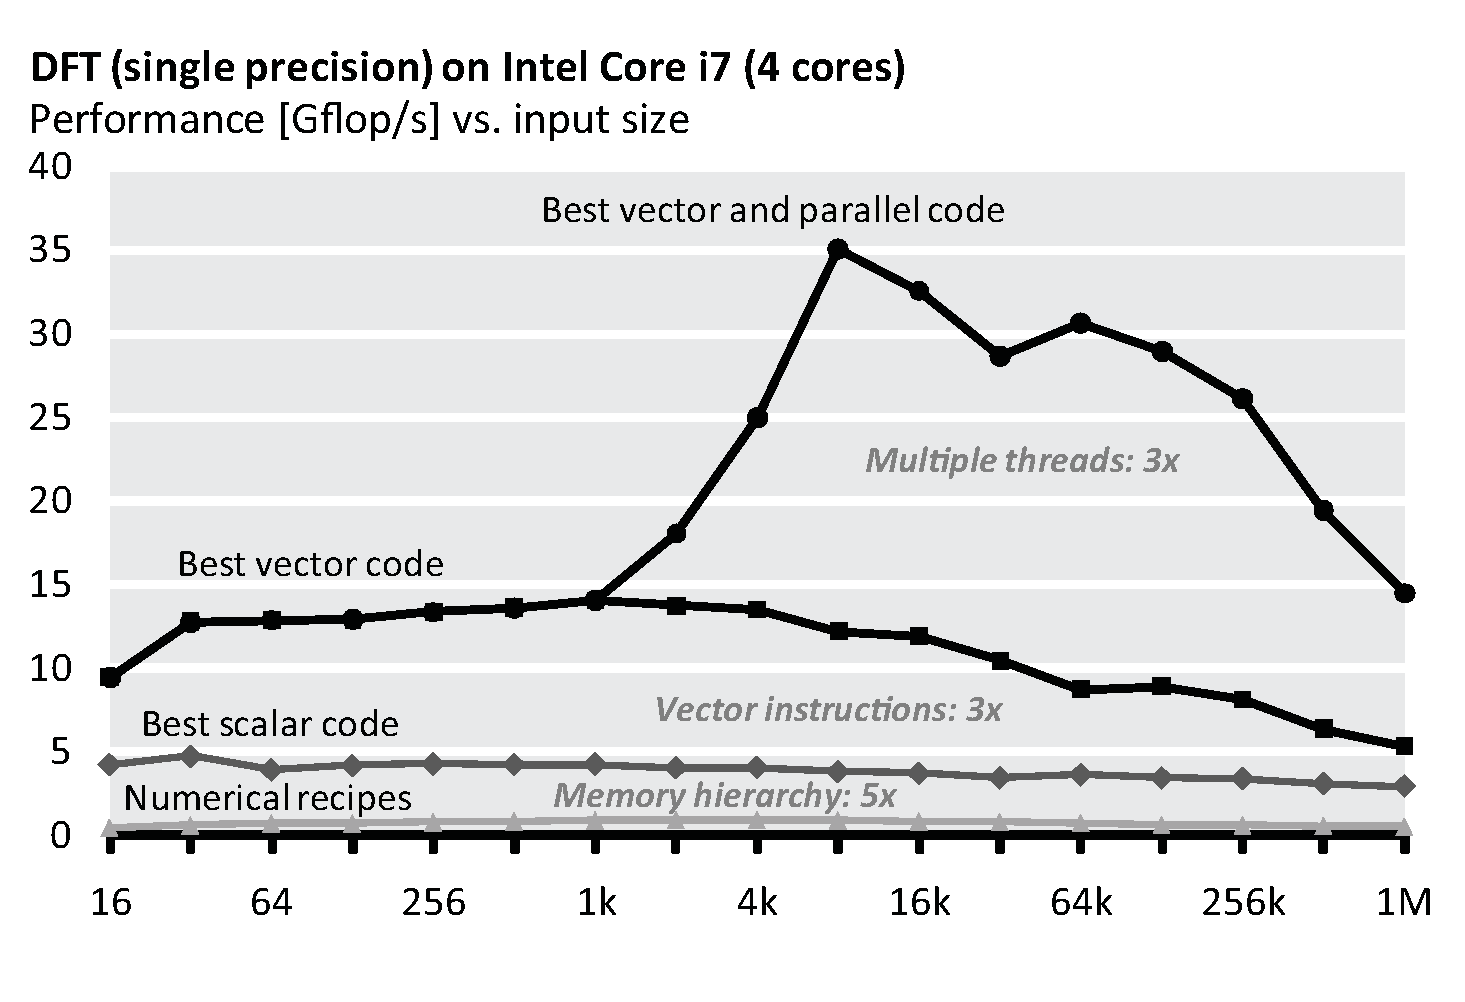
\includegraphics[scale=0.33]{dft-performance.eps}
%  \caption{Performance of four single precision implementations of the
%  discrete Fourier transform. The operations count is roughly the
%  same. {\em The labels in this plot are too small.}\label{fftperf}}
%\end{figure}